\newpage
\chapter{Оператори за контрол на изпълнението и потребителски функции}
\label{chapter05}

С процеса на усвояване на софтуерния продукт R всеки потребител установява, че някои команди биват повтаряни многократно. Това навежда на мисълта, че тези команди може да бъдат групирани и съхранени като програмен скрипт (модел на експеримента). Основното предимство на такава организация е възможността един и същи модел да бъде използван са множество експерименти. Второто предимство е, че моделът може да бъде разменян между различни потребители, които работят над същата задача или сходни задачи. Езикът R е в групата на интерпретивните програмни езици, където се намира и програмният език JavaScript. За потребителите познаващи JavaScript, някои конструкции в R биха били изключително познати. 

Скриптовете на R се записват в обикновени текстови файлове с .r разширение, както примерният файл на адрес:

\begin{lstlisting}[caption=Адрес на примерен R скрипт, label=listing0074]
https://raw.githubusercontent.com/TodorBalabanov/Statistical-Data-Processing-with-R/master/code/example0001.r
\end{lstlisting}

Може да се пише с текстов редактор по избор на потребителя, но може да се използва и текстовия редактор към продукта (Фиг. \ref{figure0025}).

\begin{figure}[h!]
  \centering
  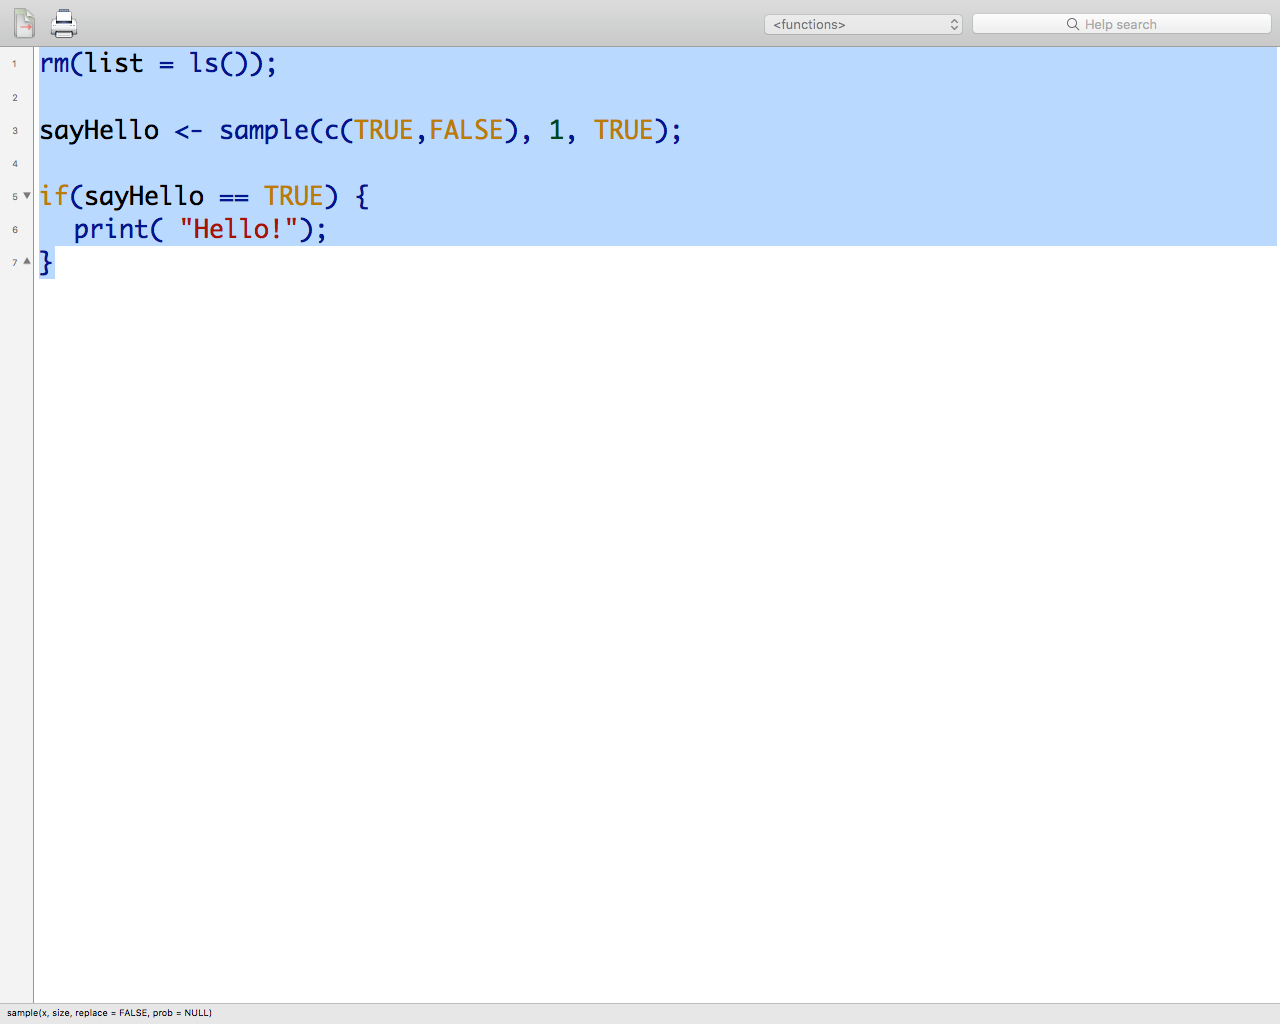
\includegraphics[width=1.0\linewidth]{pic0025}
  \caption{Текстов редактор към продукта R}
\label{figure0025}
\end{figure}
\FloatBarrier

Най-бързият начин за стартиране на скрипта е чрез менюто на вградения текстов редактор Edit->Execute (Фиг. \ref{figure0026}). 

\begin{figure}[h!]
  \centering
  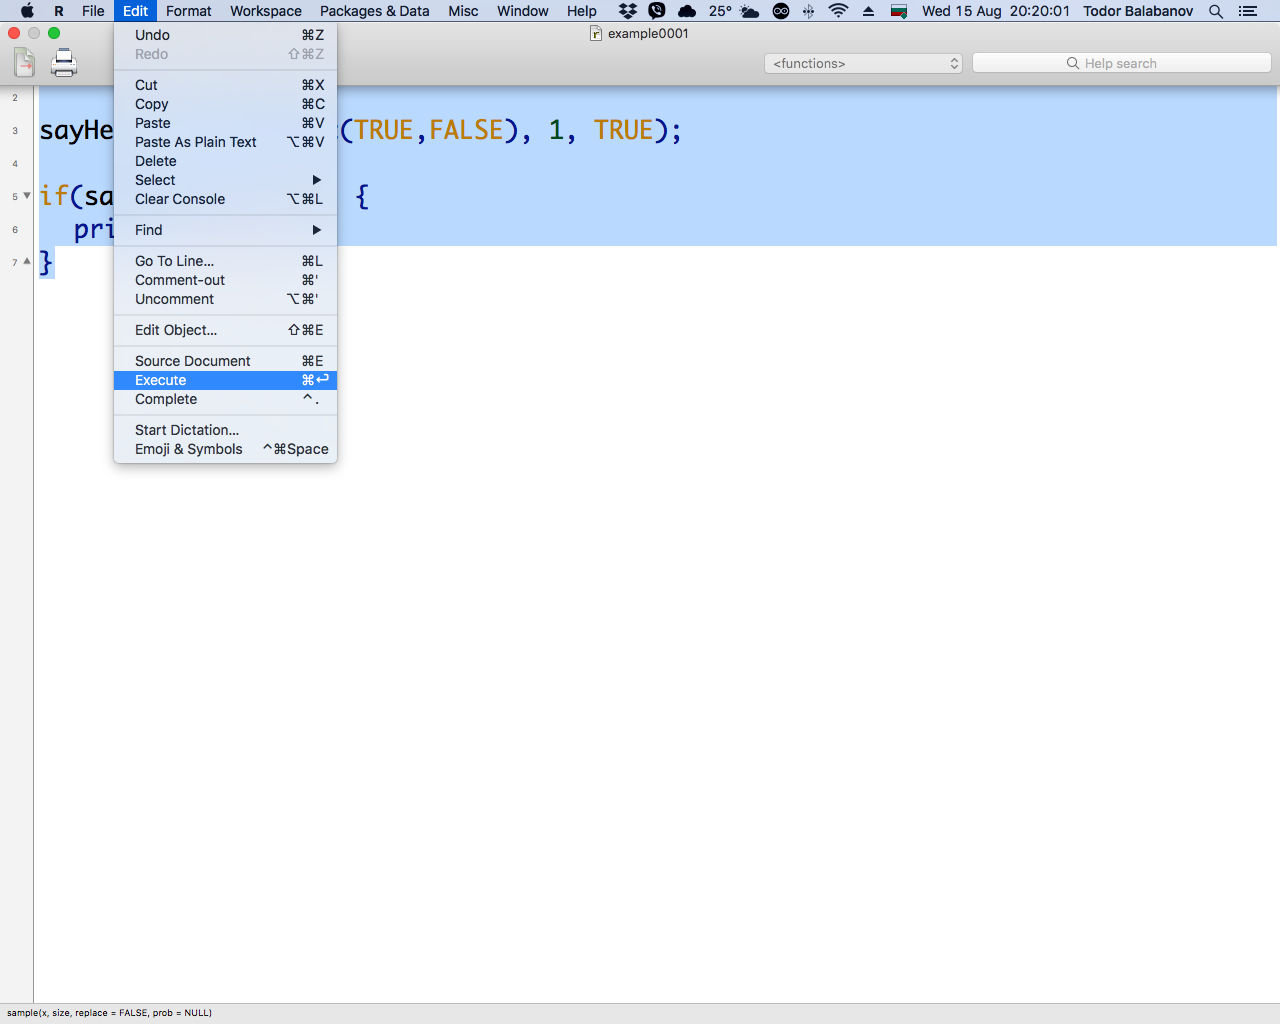
\includegraphics[width=1.0\linewidth]{pic0026}
  \caption{Стартиране на R скрипт}
\label{figure0026}
\end{figure}
\FloatBarrier

Съществено е целият текст на скрипта да бъде маркиран, тъй като командният интерпретатор е оптимизиран в режим за изпълнение на команда по команда. Когато целият скрипт е маркиран се изпълняват, една след друга, всички команди.

\begin{figure}[h!]
  \centering
  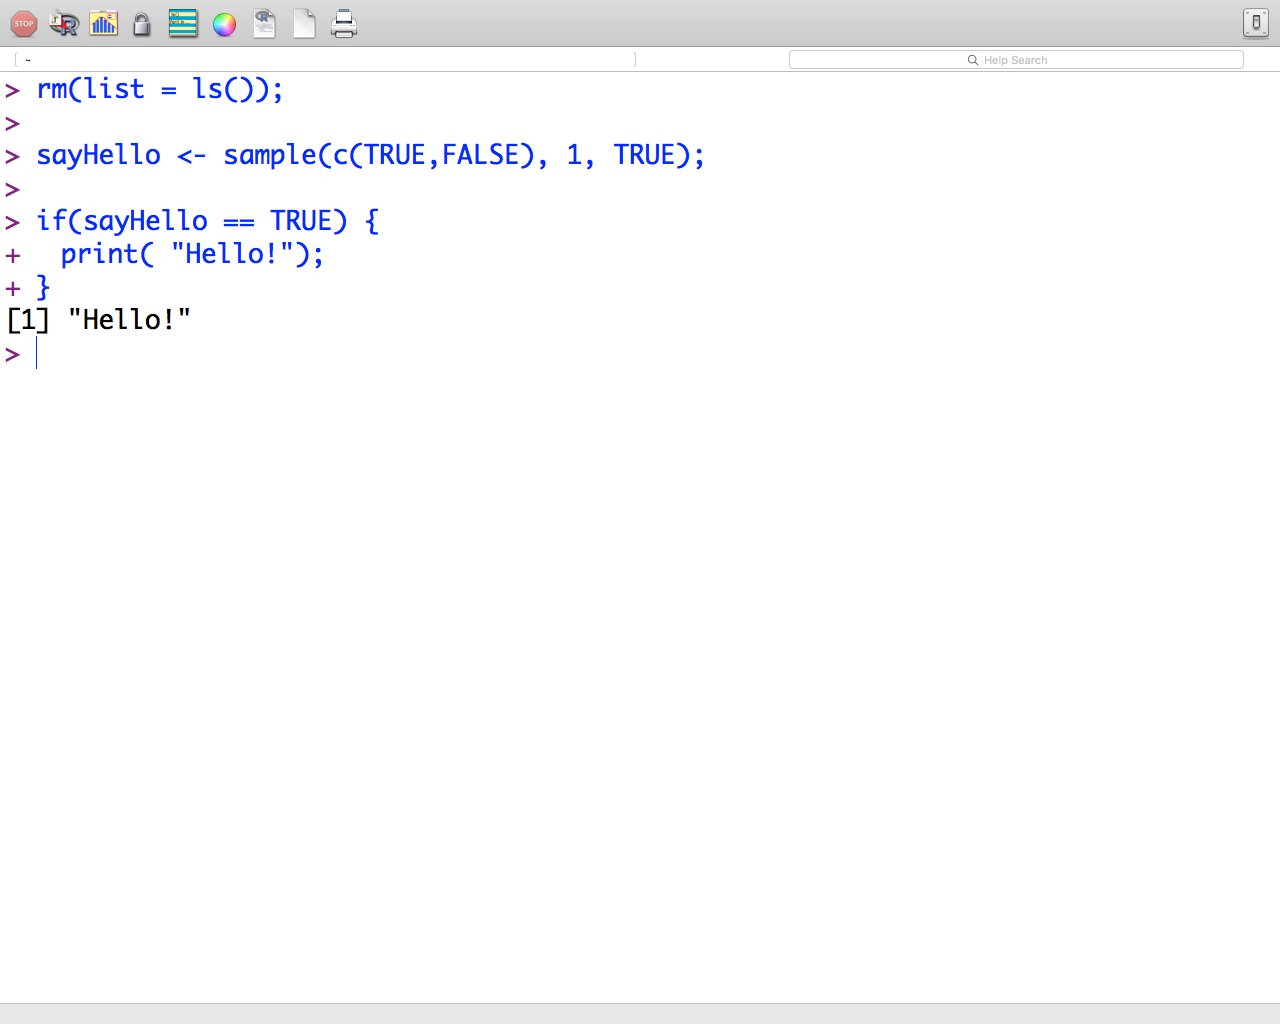
\includegraphics[width=1.0\linewidth]{pic0027}
  \caption{Резултат от изпълнението на R скрипт}
\label{figure0027}
\end{figure}
\FloatBarrier

Резултатът от изпълнението на R скрипта се наблюдава в командния интерпретатор на продукта (Фиг. \ref{figure0027}) и изглежда точно както би трябвало командите да се въведат, на ръка, ако не бяха заредени от скриптов файл.

Програмните скриптове се състоят от последователни инструкции, но с подходящи оператори за преход или повторение изпълнението на командите може да протече в различен от линейния ред. Тази група оператори се нарича оператори за контрол на изпълнението. Общата конструкция на операторите е заглавна част (ключова дума и условие) и тяло. 

\section{Оператори за преход}

Операторите за условен преход променят изпълнението на скрипта в зависимост от логическо или числено условие. От там идва и названието им. В тази група оператори попадат if, else и switch.

В заглавните части на операторите за преход може да се проверява само едно условие или да се проверяват цяла група от условия (логически изрази). За тази цел в R има логически операции като „И“ (операции \& и \&\&) и „ИЛИ“ (операции | и ||). При дойната форма на операциите се сравнява само по една стойност от двете страни (не са векторизирани), докато при единичната форма се сравняват елемент по елемент в множества от елементи от двете страни. Поради тази причина двойната форма е полезна при if оператора, а единичната форма се изисква при ifelse конструкцията. Друга много важна разлика между единичната и двойната форма е в начина по който се изчисляват изразите от двете страни на операцията. При единичната форма задължително се изчисляват и двата операнда, независимо дали това действително е нужно. При двойната форма се изчисляват само тези операнди, които са достатъчни за да определят финалният резултат от пресмятането на логическия израз. Тази разлика в използването на логическите операции може да се окаже изключително съществена, когато операндите са функции връщащи логическа стойност. В случаите когато е ненужно някой от операндите да се изчисли, тъй като другите вече са определили резултата, то част от функциите няма да бъдат извикани. С помощта на логическите операции могат да се построят много сложни логически изрази, при които важат общите правила за приоритет на операциите, както и възможността приоритетът да се променя, чрез подходящо поставяне на скоби. 

\subsection{Оператор за условен преход}

Дори чисто исторически в програмните езици един от първите оператори за преход е оператора за условен преход (if оператор). 

\begin{lstlisting}[caption=Оператор за условен преход if, label=listing0075]
sayHello <- sample(c(TRUE,FALSE), 1, TRUE);

if(sayHello == TRUE) {
	print( "Hello!" );
}

print( "Bye!" );
\end{lstlisting}

Операторът за условен преход използва ключовата дума if (Листинг \ref{listing0075}), а в заглавната му част се записва израз пресмятан до лигическа стойност TRUE или FALSE. Смисълът на оператора if е, че тялото му бива изпълнено единствено ако изчислението на израза в заглавната част доведе до стойност TRUE. Ако изразът в заглавната част бъде изчислено до стойност FALSE, тялото на оператора се пропуска и изпълнението на програмата продължава след него.

В примерът от листинг \ref{listing0075} променливата sayHello получава една случайна логическа стойност (TRUE или FALSE), като двете възможности за равно вероятни. На следващият ред операторът if изписва "Hello!" или го пропуска и изписва "Bye!". Скриптът трябва да се стартира няколко пъти за да се наблюдава ефекта от случайния избор на стойност за променливата sayHello.

\subsection{Алтернатива при условен преход}

В множество ситуации, освен основна алтернатива за оператора if, е необходимо да има и допълнителна алтернатива, която да се изпълни при резултат от логическия израз FALSE. За тази цел конструкцията на оператора if може да се разшири с добавяне на else конструкция (Листинг \ref{listing0076}).

\begin{lstlisting}[caption=Оператор за условен преход if-else, label=listing0076]
sayHello <- sample(c(TRUE,FALSE), 1, TRUE);

if(sayHello == TRUE) {
	print( "Hello!" );
} else {
	print( "Hi!" );
}

print( "Bye!" );
\end{lstlisting}
Конструкцията else е контекстно зависима и поради тази причина може да се използва единствено в комбинация с конструкцията на оператора if. В примерния код от листинг \ref{listing0076} в половината от случаите на конзолата ще се изпише "Hello!", а в другата половина "Hi!".

\subsection{Каскада от условни преходи}

Условният преход ограничава до две възможности, но практиката понякога налага да се избират повече алтернативи. В такава ситуация може да се използва каскада от if-else конструкции (Листинг \ref{listing0077}).

\begin{lstlisting}[caption=Каскада от if-else, label=listing0077]
sayHello <- sample(c(0,1,2), 1, TRUE);

if(sayHello == 0) {
	print( "Hello!" );
} else if(sayHello == 1) {
	print( "Hi!" );
} else if(sayHello == 2) {
	print( "Yoo!" );
} else {
	print( "Error!" );
}

print( "Bye!" );
\end{lstlisting}

Недостатък на каскадните проверки е, че всяко условие трябва да бъде проверявано по отделно. Каскадата може да завършва с else конструкция, но тя не е задължителна. 

R предлага ifelse оператор, който много прилича на if конструкцията в Microsoft Excel (Листинг \ref{listing0078}) и сериозно се различава от if-else оператора. Една от най-силните страни на ifelse конструкцията е, че тя е векторизирана и може да се прилага над група елементи едновременно. 

\begin{lstlisting}[caption=Функцията ifelse, label=listing0078]
ifelse(sample(c(FALSE,TRUE), 1, TRUE), "Yes", "No")

ifelse(c(1,1,0,1,0,1)==1, "Yes", "No")
\end{lstlisting}

\subsection{Оператор за многовариантен избор}

Писането на каскадни конструкции от типа if-else може да бъде твърде неудобно и поради тази причина съществува switch конструкцията (Листинг \ref{listing0079}).

\begin{lstlisting}[caption=Конструкция за многовариантен избор switch, label=listing0079]
switch(sample(c("a","b","c","d","e"),1,TRUE), "a"="one", "b"="two", "c"="three", "d"="four", "other")
\end{lstlisting}

В примерния код на случаен принцип се избира една буква от пет възможни, след което се проверяват четири алтернативи и последна опция за else условие. 

Първият аргумент е стойността която ще се проверява, а след това са изброени алтернативните възможности. Последната стойност, ако не й е зададена стойност за проверка, служи за отговор, коато нито една от алтернативите не е била определена. 

\section{Оператори за цикъл}


